\documentclass{article}
\usepackage[margin=1in]{geometry}
\usepackage{fancyhdr}
\usepackage{graphicx}
\usepackage{vhistory}
\usepackage[parfill]{parskip}
\graphicspath{{./}}

% Set fancy looking header/footer and move page number to the right
\pagestyle{fancy}
\fancyhead{}
\fancyfoot{}
\fancyfoot[R]{\thepage}

\title{}
\author{}
\date{}

\begin{document}

    % For large document with titlepage:
    \pagenumbering{gobble}
    \begin{titlepage}
    \begin{center}
        \vspace*{1cm}

        \Huge
        \textbf{User's Guide for Cloud Backup}

        \vspace{.5cm}
        \LARGE
        Captain CyBeard: Neil Before Us

        \vspace{1cm}

        \textbf{Ryan Breitenfeldt \textbar\ Noah Farris\\ Trevor Surface \textbar\ Kyle Thomas}

        \vspace{.2cm}
        \Large
        May 4, 2020

        \vspace{2cm}
        
\includegraphics[scale=1]{logo}

        \vfill

        Washington State University Tri-Cities\\
        CptS 423 Software Design Project 2

    \end{center}
\end{titlepage}



    \tableofcontents
    \listoffigures

    \newpage
    \begin{versionhistory}
        \vhEntry{0.2}{10.10.2019}{RB NF TS KT}{Filled in Environment \& Operation sections}
        \vhEntry{0.1}{09.27.2019}{KT}{Document Creation}
    \end{versionhistory}
    \newpage

    \pagenumbering{arabic}
    \section{Introduction}
    % Doc purpose, class, school, what the req specs does

    % What the rest of the document has (sections)
		
    \section{Background}
    % About Cypherpath and their resiliency platform
    % Explain what this application is supposed to solve at a high, nontechnical level

    \section{Overview}
    % How the application will solve the problem, what environment it will run in, language, platform, etc
    % Overview of what it will do

    \section{Environment}
    The environment that the software will preside in consists of modules to interact with \textbf{VMWare}, 
    \textbf{AWS}, other virtual machine platforms and will also be interacting with authentication modules for those
    various platforms. The user will interact with the API's of these cloud services and authentication
    methods through a Django Web App. Lastly, the environment will consist of the application storing the selected
    virtual machines onto the user's local machine.

    %%%%%%%%%%%%%%% DIAGRAM STILL NEEDS TO BE FIXED!!! %%%%%%%%%%%%%%%%%%%%%%%%%%
    \begin{figure}[h]
    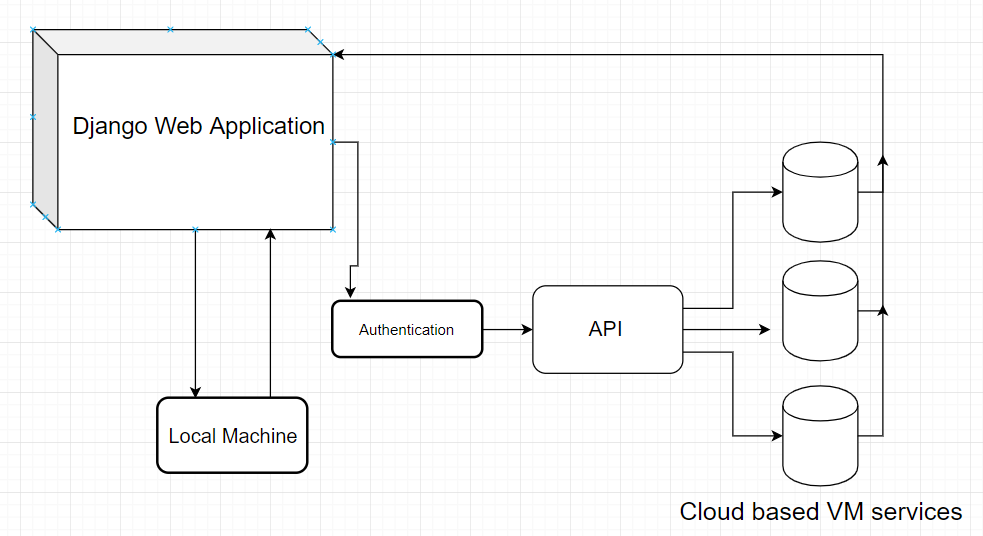
\includegraphics[scale=.7]{diagram}
        \caption{The application environment}
    \end{figure}
    %%%%%%%%%%%%%%% DIAGRAM STILL NEEDS TO BE FIXED!!! %%%%%%%%%%%%%%%%%%%%%%%%%%

        \subsection{VMWare (VSphere)}

            \subsubsection{API'S}
            Use VMWare API that looks at file structs.

            Example URL:

            \subsubsection{Download Protocol}
            Call downloads to download to local machine.

        \subsection{AWS}
            \subsubsection{API'S}
            Use AWS API that looks at file structs.

            \subsubsection{Download Protocol}
            Call download API to download to local machine.

        \subsection{Authentication}
            \subsubsection{VMWare Auth (SAML)}
            Use specific authorization based on the VMWare standard.

            \subsubsection{AWS Auth}
            Use specific authorization based on the AWS standard.

        \subsection{Web Page}
            \subsubsection{Django}
            Provide input box for URL: should also provide login and logout usage.

        \subsection{Download Structure}

        \subsection{Database?}

    \section{Operation}
    In the following sections the operation of the application will be described, including starting the application
    (invocation), the commands the application uses and finally, how to close or terminate the application.

        \subsection{Invocation}
            \subsubsection{Web Application}

        \subsection{Commands}
            \subsubsection{Download}
            
            \subsubsection{Load File Structure}

            \subsubsection{Error Catching}

            \subsubsection{Authentication}

        \subsection{Termination}
            \subsubsection{Logout User}

            \subsubsection{Closing Application}

    \section*{References}
    % Reference the project plan?
    % Possibly reference documentation to the various API's?

    \appendix
    \section{Appendix}
    % Sample files, if any?
    % Maybe a sketch of the general page layout?

\end{document}
